\documentclass{beamer}
\usepackage{graphicx,amsmath,amsfonts,amssymb,listings,tikz}
\usepackage{bm}
\usepackage{multimedia}
\usetheme{Montpellier}
%\usecolortheme{beaver}
\beamerdefaultoverlayspecification{<+->}
\definecolor{mygray}{rgb}{0.92,0.92,0.92}

\begin{document}

\section{Introduction}
\title{A Fully Adaptive Block-Structured Multiresolution Scheme for
Reactive Flows}
\author{Brandon Gusto} %
\institute{Dept. of Scientific Computing \\ Florida State University}
\date{\today}
\frame{\titlepage}

\section{Introduction}

\begin{frame}{Introduction}
    Many engineering applications depend on numerically solving systems of conservation laws of the form
    \begin{equation}
    \begin{cases}
      u_{t} + f(u)_{x} = s(u) \\
      u(x,0) = u_{0}(x),
    \end{cases}
    \label{claw}
    \end{equation}
    where $x \in \Omega$ and $t \in [t_{0},t_{f}]$.
    Volume averages are defined for each cell $I_{i} =
    \left[x_{i-1/2},x_{i+1/2}\right]$,
    \begin{equation}
        \overline{u}_{i}(t) = \frac{1}{\Delta x} \int_{x_{i-1/2}}^{x_{i+1/2}} u(\xi,t) d \xi,
    \end{equation}
\end{frame}

\begin{frame}{Discretization}
    The governing equations are cast into the semi-discrete conservative form,
    \begin{equation}
        \frac{d \overline{u}_{i}(t)}{dt} = L(\overline{\bm{u}}) = -\frac{1}{\Delta x} \left( \hat{f}_{i+1/2} -
        \hat{f}_{i-1/2} \right) + \overline{s}_{i},
        \label{ode}
    \end{equation}
    where $\overline{s} = \frac{1}{\Delta x} \int_{x_{i-1/2}}^{x_{i+1/2}} s(u) d
    \xi$, and the numerical flux is evaluated as
    \begin{equation}
        \hat{f}_{i\pm1/2} = \hat{f}(\overline{u}^{-}_{i\pm1/2}, \overline{u}^{+}_{i\pm1/2}).
    \end{equation}
\end{frame}

\begin{frame}{Riemann problem}
    \begin{figure}
        \center
        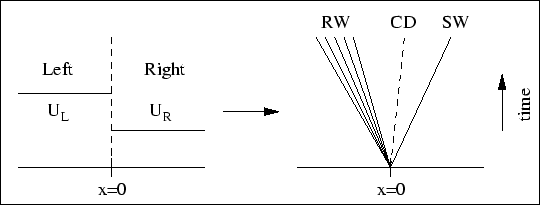
\includegraphics[width=0.8\textwidth]{riemann.png}
    \end{figure}
\end{frame}

\begin{frame}{Time integration}
    This system of ODEs is evolved forward in time
    \begin{equation}
        \overline{\bm{u}}^{n+1} = \overline{\bm{u}}^{n} + \Delta t \sum_{j=1}^{s} b_{j}
        \bm{k}_{j},
    \end{equation}
    where the stages $k_{j}$ are solved either implicitly or explicitly.
\end{frame}

% provide example that motivates AMR
\begin{frame}
    \frametitle{Motivation for non-uniform refinement}
\end{frame}

\begin{frame}{Adaptive mesh refinement}
    These equations are typically solved on non-uniform mesh spacing:
    % should setup two-column environment here...
    \begin{itemize}
        \item<2-> refinement is associated with localized features
        \item<3-> some type of estimator of the local error is needed
        \item<4-> typically a collection of cells (a block) is refined for efficiency
        \item<5-> blocks introduce inherent ``overresolution" in some regions of the mesh
    \end{itemize}
\end{frame}

\begin{frame}
    \frametitle{Constraints of AMR}
\end{frame}

%\section{Computing Limitations}
%\begin{frame}{Computing limitations}
%    \begin{figure}
%        \center
%        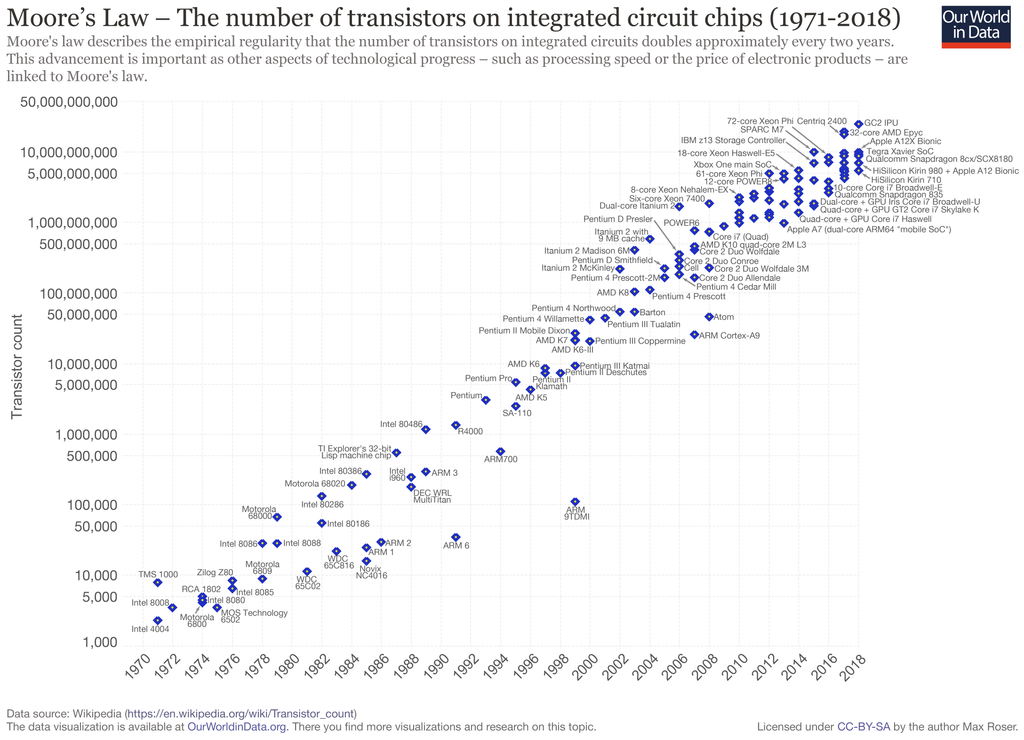
\includegraphics[width=0.8\textwidth]{moore.png}
%    \end{figure}
%\end{frame}

\section{Multiresolution representation}

\begin{frame}{Mesh hierarchy}
    Define multiple levels of representation of the discrete data
    \begin{equation*}
        \bm{\mathcal{G}}_{l} = \left\{ x_{i}^{l} \right\}_{i=0}^{N_{l}}, \text{ }
        \text{ } \text{ } \text{ } x_{i}^{l} = i \cdot \Delta x_{l}, \text{ }
        \text{ } \Delta x_{l} = 2^{L-l} \cdot \Delta x_{L}, \text{ } \text{ } N_{l} = N_{L}
        / 2^{L-l},
    \end{equation*}
    where $\Delta x_{l}$ and $N_{l}$ denote the cell width and number of cells,
    respectively, on level $l$.
    The index space of cells on each level of the hierarchy is denoted by
    $\bm{\mathcal{I}}^{l} = \left\{ 1,\dots,N_{l} \right\}$.
\end{frame}

\begin{frame}{Decomposition}
    \begin{enumerate}
        \item[] \textit{Project:} The cells at level $l+1$ are projected
            by means of averaging, onto the coarser grid
            level $l$. The projection is defined by a linear operator
            which performs the mapping $\bm{P}_{l+1}^{l} : \overline{\bm{u}}^{l+1}
            \mapsto \overline{\bm{u}}^{l}$. 
        \item[] \textit{Predict}: Cell averages at level $l+1$
            are predicted by an average-interpolating polynomial constructed
            of cells on level $l$. The prediction operator performs
            the mapping $\bm{P}_{l}^{l+1} : \overline{\bm{u}}^{l} \mapsto
            \tilde{\bm{u}}^{l+1}$. 
    \end{enumerate}
\end{frame}

\begin{frame}{Project}
    Coarsening/projection is done via
    \begin{equation}
        \overline{u}^{l}_{i} = \left( \bm{P}_{l+1}^{l}
        \overline{\bm{u}}^{l+1} \right)_{i} = \frac{1}{2} (
        \overline{u}^{l+1}_{2i-1} + \overline{u}^{l+1}_{2i} ), \quad \forall
        i \in \bm{\mathcal{I}}^{l}.
    \end{equation}
\end{frame}

\begin{frame}{Predict}
    Prediction is done using average-interpolating polynomials, with
    $m\in\{0,1\}$,
    \begin{equation*}
        \tilde{u}_{2i-m}^{l+1} = \overline{u}_{i}^{l} - (-1)^{m} \sum_{p=1}^{s} \gamma_{p} \left(
            \overline{u}^{l}_{i+p} - \overline{u}^{l}_{i-p} \right), \quad \forall i \in
            \bm{\mathcal{I}}^{l}.
        \label{prediction}
    \end{equation*}
\end{frame}

\begin{frame}{Difference information and thresholding}
    We compute a difference between the true value at the higher resolution
    $l+1$, and its prediction,
    \begin{equation}
        d^{l}_{i} = \overline{u}^{l+1}_{2i} - \tilde{u}^{l+1}_{2i}, \quad \forall i \in \bm{\mathcal{I}}^{l}.
    \end{equation}
    Then we can eliminate small detail coefficients (where solution is smooth
    enough),
    \begin{equation}
        \tilde{d}^{l}_{i} =
            \begin{cases}
                d^{l}_{i}, \text{ } \text{if} \text{ } |d^{l}_{i}| > \varepsilon \\
                0, \text{ } \text{if} \text{ } |d^{l}_{i}| \leq
                \varepsilon.
            \end{cases}
    \end{equation}
    Then reconstructing field is done by
    \begin{equation*}
        \overline{u}^{l+1}_{2i} = \tilde{u}^{l+1}_{2i} + \tilde{d}^{l}_{i}.
    \end{equation*}
\end{frame}

% should show simple example of multiresolution compression of function
\begin{frame}
    \frametitle{Multiresolution compression of function}
\end{frame}

\section{Grid Adaptation}

% describe mask
\begin{frame}{Grid adaptation}
    (MOVIE)
\end{frame}

% describe buffer zone
\begin{frame}
    \frametitle{Buffer region}
\end{frame}

% give source terms their own slide
\begin{frame}{Adaptive flux and source computations on blocks}
    Where the mask is not active (solution is smooth enough), we can also
    replace redundant flux calculations with interpolation,
    \begin{equation}
        \hat{f}_{2i+1}^{l+1} \approx \sum_{p=1}^{s+1} \beta_{p} \left(
        \hat{f}^{l}_{i-p+1} + \hat{f}^{l}_{i+p} \right).
    \end{equation}
    We can do the same for the source terms,
    \begin{equation}
        \overline{s}_{2i-m}^{l+1} \approx \overline{s}_{i}^{l} - (-1)^{m} \sum_{p=1}^{k} \gamma_{p} \left(
            \overline{s}^{l}_{i+p} - \overline{s}^{l}_{i-p} \right).
    \end{equation}
\end{frame}

% discuss possible load-balancing using multiresolution info
\begin{frame}
    \frametitle{Load balancing}
\end{frame}

\section{Results}

\begin{frame}{Two interacting blast waves}
  \begin{figure}
    \center
    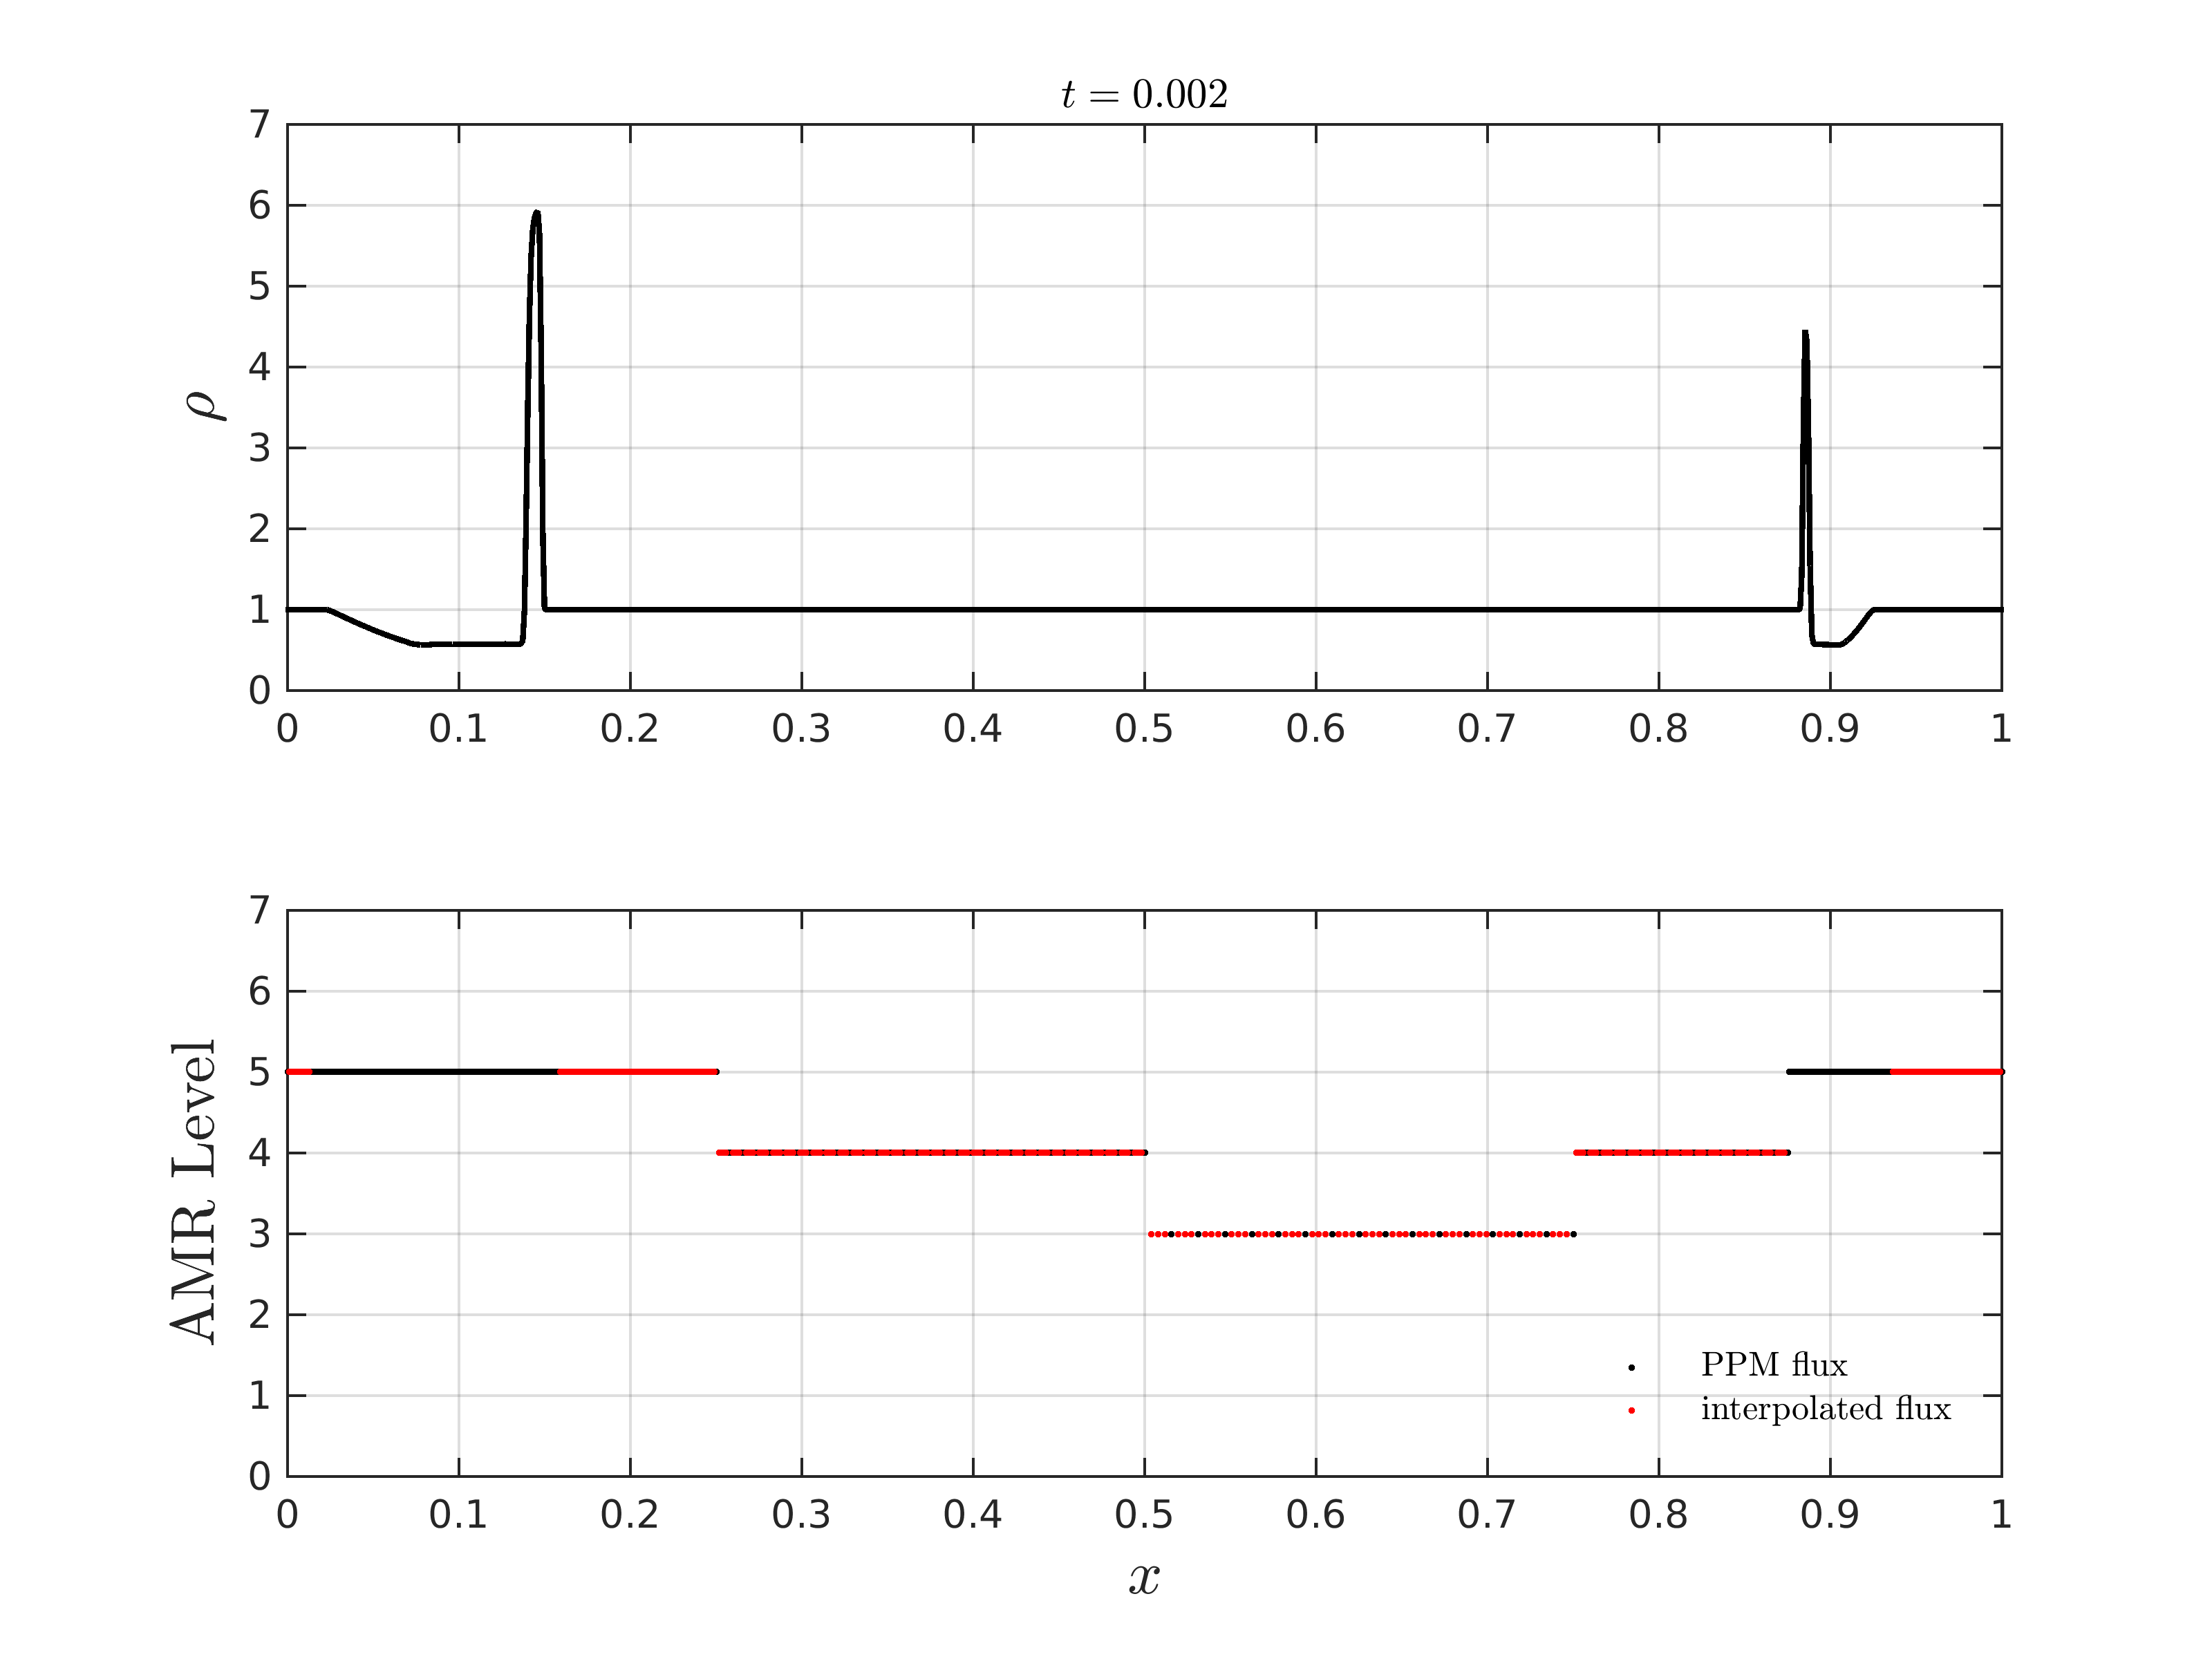
\includegraphics[scale=0.4]{blast2_early.png}
  \end{figure}
\end{frame}

\begin{frame}{Laminar flame}
  \begin{figure}
    \center
      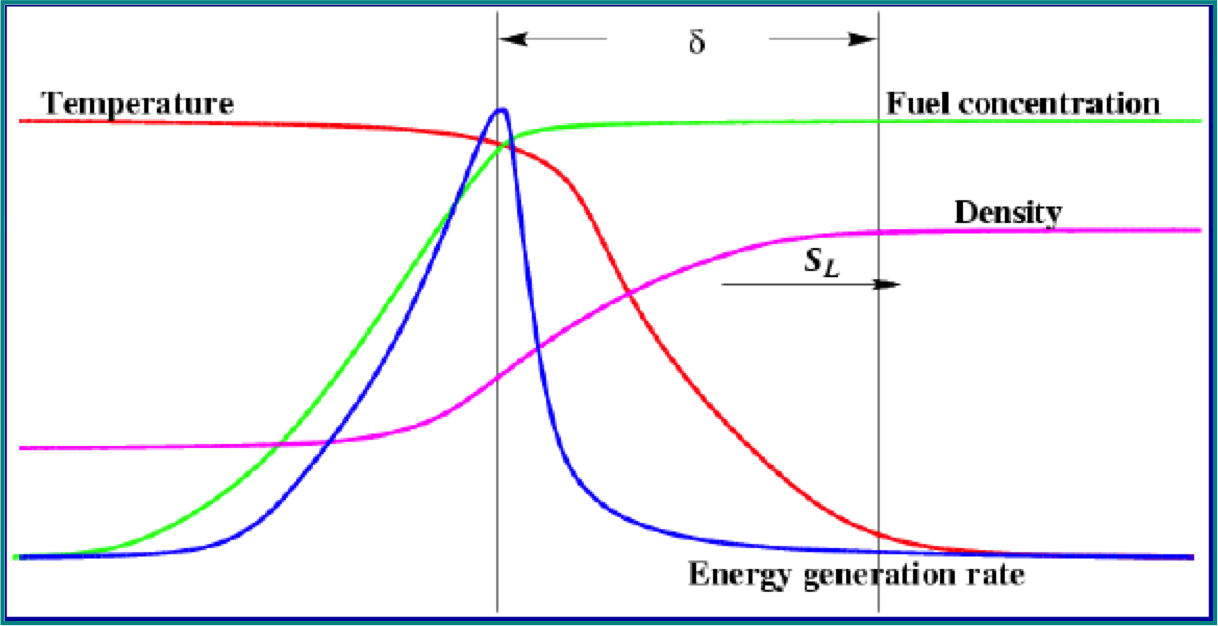
\includegraphics[width=0.75\textwidth]{laminarflame.png}
  \end{figure}
\end{frame}

\begin{frame}{Nuclear burning}
  \begin{figure}
    \center
      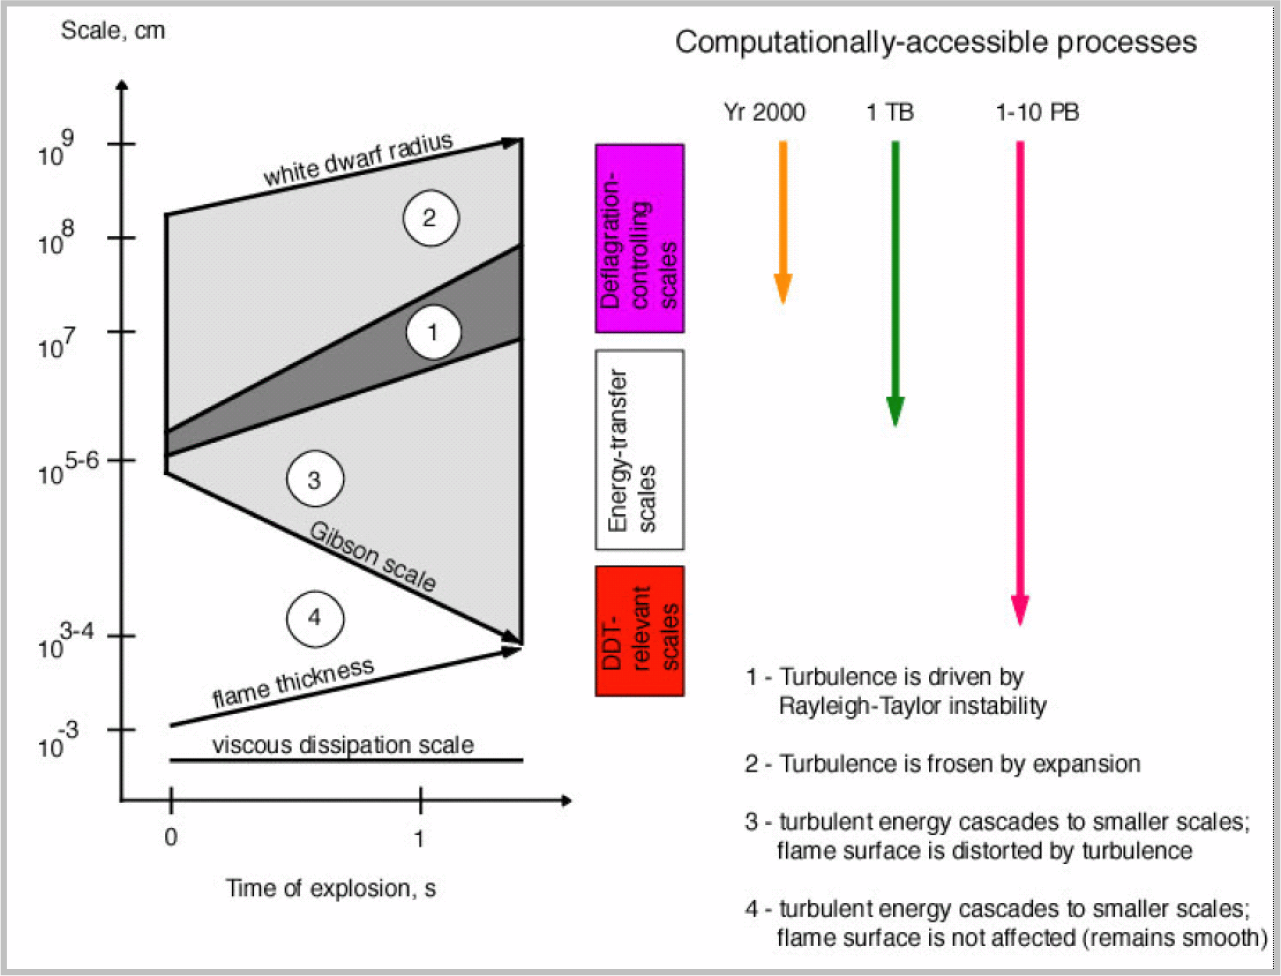
\includegraphics[width=0.75\textwidth]{scales.png}
  \end{figure}
\end{frame}

\end{document}
